\documentclass[12pt,a4paper,openright,twoside]{book}
\usepackage[utf8]{inputenc}
\usepackage{disi-thesis}
\usepackage{code-lstlistings}
\usepackage{notes}
\usepackage{shortcuts}
\usepackage{acronym}

\school{\unibo}
\programme{Corso di Laurea Triennale in Ingegneria e Scienze Informatiche}
\title{Da MIT Proto a Collektive: Trasposizione di esempi di programmazione aggregata in un DSL in Kotlin.}
\author{Andrea Cecchini}
\date{\today}
\subject{Programmazione ad Oggetti}
\supervisor{Prof. Danilo Pianini}
\cosupervisor{Dott. Angela Cortecchia}
\session{III}
\academicyear{2024-2025}

% Definition of acronyms
\acrodef{AC}{Programmazione Aggregata}
\acrodef{FC}{Field Calculus}
\acrodef{HFC}{Higher-Order Field Calculus}
\acrodef{XC}{eXchange Calculus}

\mainlinespacing{1.241} % line spacing in mainmatter, comment to default (1)

\begin{document}

\frontmatter\frontispiece

\begin{abstract}	
Max 2000 characters, strict.
\end{abstract}

\begin{dedication} % this is optional
Optional. Max a few lines.
\end{dedication}

%----------------------------------------------------------------------------------------
\tableofcontents   
\listoffigures     % (optional) comment if empty
\lstlistoflistings % (optional) comment if empty
%----------------------------------------------------------------------------------------

\mainmatter

%----------------------------------------------------------------------------------------
\chapter{Introduzione}
\label{chap:introduzione}
%----------------------------------------------------------------------------------------



\section{Contesto}
\label{sec:contesto}

\subsection{Programmazione Aggregata}
\label{sec:programmazioneaggregata}

\subsection{Field Calculus e Higher Order Calculus}
\label{sec:fieldcalculus}

\subsubsection{Campo computazionale}
\label{sec:campo_computazionale}

\subsubsection{Dinamica Temporale e Stato}
\label{sec:dinamicatemporale}

\subsubsection{Interazione Spaziale e Vicinato}
\label{sec:interazionespaziale}

\subsubsection{Restrizione dello Spazio e Condizionali}
\label{sec:restrizionespazio}

\subsection{Share e XC Calculus}
\label{sec:sharandexc}

\newpage
\section{Motivazione}
\label{sec:motivazione}

\subsection{MIT Proto}
\label{sec:mitproto}

\subsection{Protelis}
\label{sec:protelis}

\subsection{Scafi}
\label{sec:scafi}

\subsection{FCPP}
\label{sec:fcpp}

\subsection{Collektive}
\label{sec:collektive}

\newpage
\section{Obiettivo}
\label{sec:obiettivo}

%----------------------------------------------------------------------------------------
\chapter{MIT-Proto}
\label{chap:mitproto}
%----------------------------------------------------------------------------------------

\section{Introduzione alla sintassi}
\label{sec:mitprotosyntax}

\section{Operatori}
\label{sec:mitprotooperators}

\section{Funzioni built-in}
\label{sec:mitprotobuiltin}


%----------------------------------------------------------------------------------------
\chapter{Collektive}
\label{chap:collektive}
%----------------------------------------------------------------------------------------

\section{Field}
\label{sec:collektivefields}

\section{Operazioni aggregate}
\label{sec:collektiveaggregateops}

\subsection{Exchange}
\label{sec:collektiveexchange}

\subsection{Neighborhood}
\label{sec:collektiveneighborhood}

\subsection{Neighboring}
\label{sec:collektiveneighboring}

\subsection{Evolve}
\label{sec:collektiveevolve}

\subsection{Share}
\label{sec:collektiveshare}

\section{Manipolazione dei Field}
\label{sec:collektivefieldmanipulation}

\section{Standard Library}
\label{sec:collektivelibrary}


%----------------------------------------------------------------------------------------
\chapter{Trasposizione di esempi da MIT-Proto a Collektive}
\label{chap:trasposizione}
%----------------------------------------------------------------------------------------

Sono qui riportati alcuni programmi prototipali originariamente realizzati in MIT-Proto 
e la loro successiva implementazione in Collektive.
%
Per ciascun esempio, vengono forniti: il codice originale, una spiegazione del suo funzionamento, 
la sua trasposizione in Collektive e alcune immagini relative alle simulazioni condotte.
% 
Le simulazioni sono state eseguite utilizzando il simulatore Alchemist \cite{alchemist}.
%
Verranno discussi i seguenti esempi:
\begin{itemize}
    \item Media Locale (\cref{sec:localaverage})
    \item Nel Cerchio (\cref{sec:incircle})
    \item Anello (\cref{sec:ring})
    \item Temperature (\cref{sec:temperature})
    \item Navigazione del Gradiente (\cref{sec:navgrad})
    \item Partizione di Voronoi (\cref{sec:voronoi})
    \item Connessione lungo l'albero di percorso minimo (\cref{sec:wire})
    \item Tracciamento (\cref{sec:track})
    \item Dinamica di uno stormo (\cref{sec:flock})
\end{itemize}

\newpage
\section{Media Locale}
\label{sec:localaverage}

In \cref{lst:localaverage} è riportato il codice MIT-Proto.
%
\lstinputlisting[
    language=Lisp,
    label={lst:localaverage},
    caption={\url{https://github.com/jakebeal/MIT-Proto/blob/master/proto/demos/local-average.proto}}
]{listings/proto/local-average.proto}
%
L'obiettivo del programma è determinare il vettore medio a partire
dai vettori associati ai nodi presenti nel vicinato.

La funzione \texttt{local-average} accetta come argomento un campo di
vettori \texttt{v}, di tre dimensioni.
%
L'espressione nel suo complesso è definita come il prodotto (\texttt{*}) di due termini distinti.
%
Il termine di destra, \texttt{(fold-hood + (tup 0 0 0) v)}, calcola la somma di tutti
i vettori locali nel vicinato. 
%
Il termine di sinistra, \texttt{(/ 1 (sum-hood 1))}, è invece responsabile del conteggio 
dei dispositivi nel vicinato e del calcolo del suo inverso.
%
Il risultato dell'espressione \texttt{local-average} è quindi formalizzato come segue:
\[
    \texttt{local-average(v)} = \frac{1}{\sum_{d \in N} 1} \cdot \sum_{d \in N} v(d)
\]
dove \(N\) rappresenta l'insieme dei dispositivi nel vicinato.

La trasposizione in Collektive è riportata in \cref{lst:localaverageck}, 
mentre in \cref{fig:local-average-simulation} è mostrata una simulazione dell'esperimento.


\lstinputlisting[
    language=Kotlin,
    label={lst:localaverageck},
    caption={\url{https://github.com/Collektive/collektive-examples/blob/master/simulation/src/main/kotlin/it/unibo/collektive/examples/localAverage/LocalAverage.kt}}
]{listings/collektive/localAverage.kt}

\begin{figure}
    \centering
    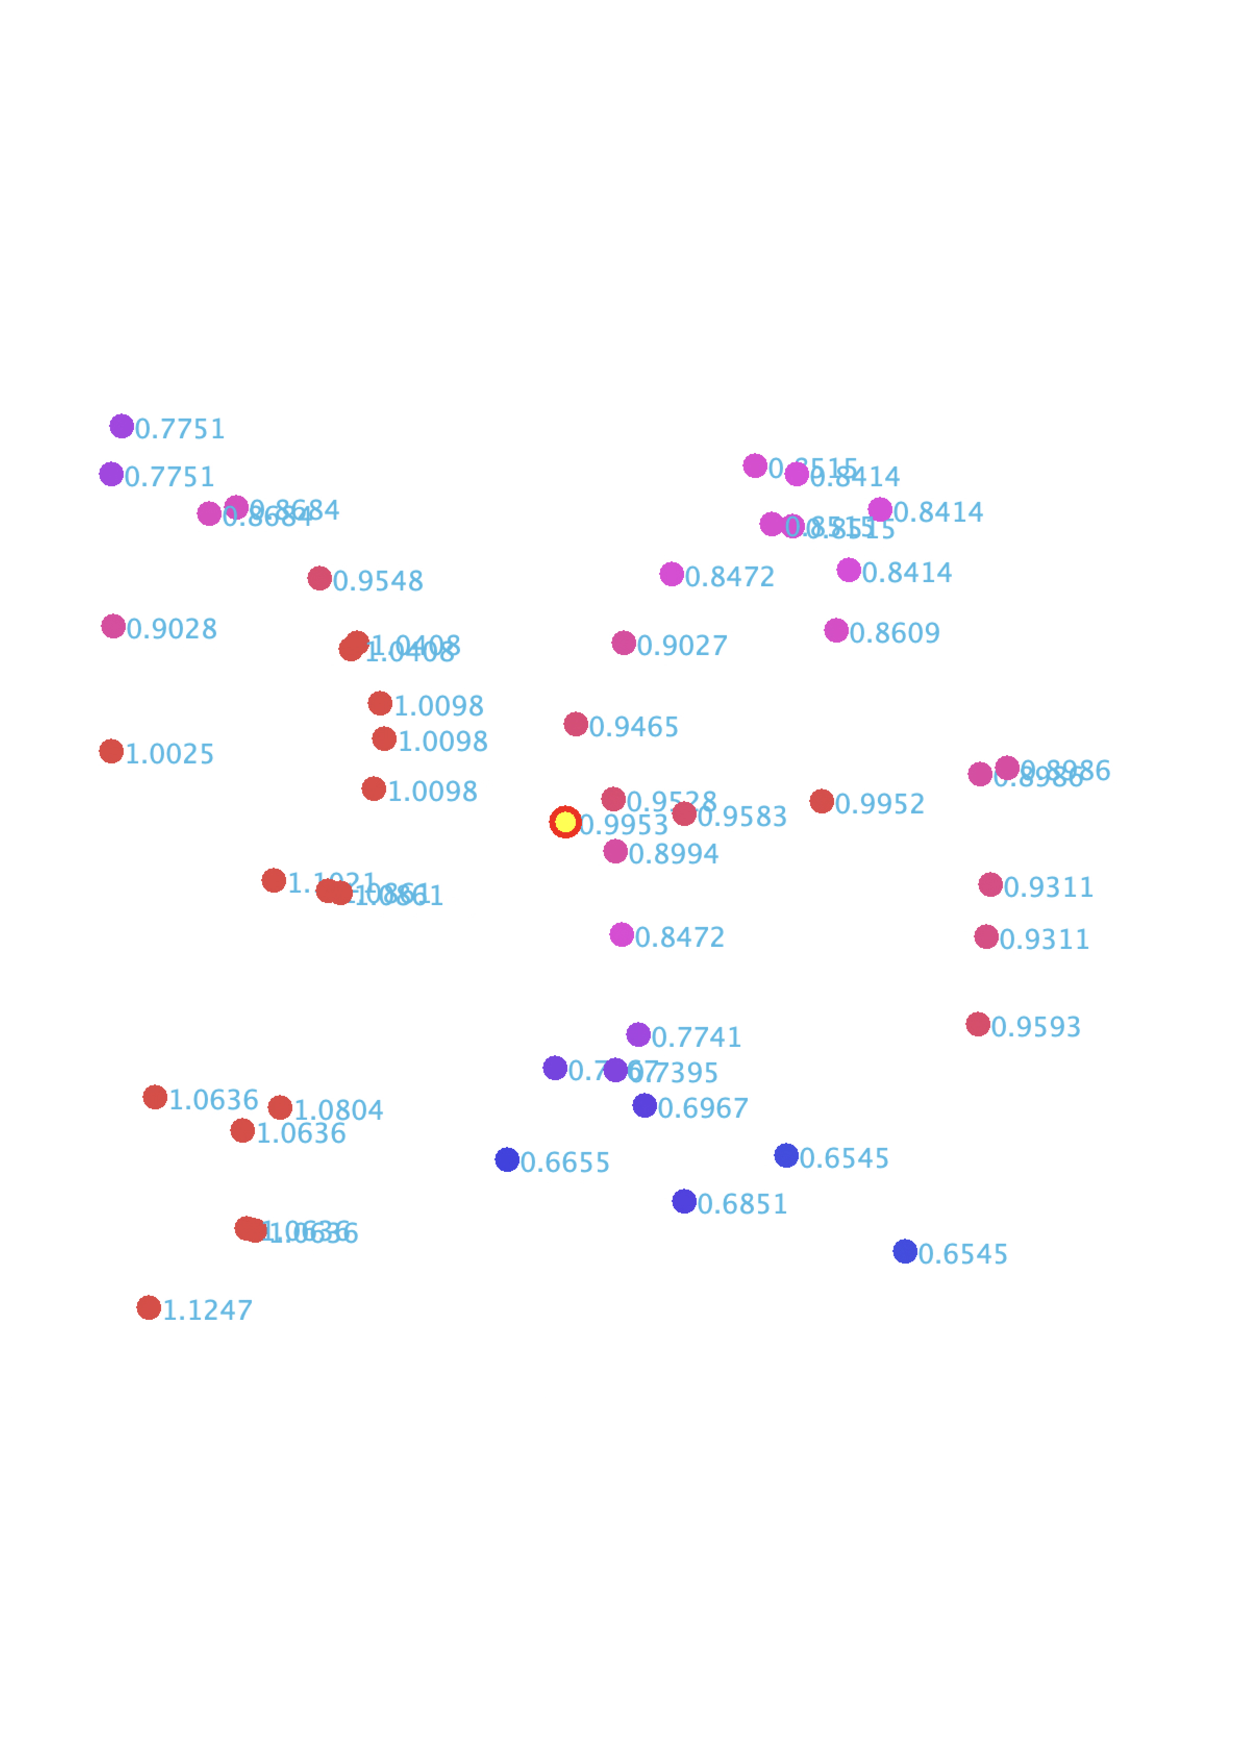
\includegraphics[width=.8\linewidth]{figures/localAverageSimulation.pdf}
    \caption{Simulazione dell'esperimento di Media Locale in Alchemist.
     I dispositivi inizializzano \texttt{v} casualmente e convergono verso il valore medio locale.
    Al vettore risultante viene applicata la norma euclidea per visualizzarlo come scalare.}
    \label{fig:local-average-simulation}
\end{figure}


\section{Nel Cerchio}
\label{sec:incircle}

In \cref{lst:incircle} è riportato il codice MIT-Proto.
%
\lstinputlisting[
    language=Lisp,
    label={lst:incircle},
    caption={\url{https://github.com/jakebeal/MIT-Proto/blob/master/proto/demos/in-circle.proto}}
]{listings/proto/in-circle.proto}
%
La funzione \texttt{in-circle} accetta come argomenti un campo booleano \texttt{o}, 
il quale identifica il nodo che funge da origine del cerchio, 
e un raggio \texttt{r}.
%
L'obiettivo del programma è determinare se un dispositivo 
si trova all'interno della regione circolare di raggio \texttt{r}
centrata nell'origine definita.
%
L'istruzione \texttt{let ((dv (- (probe (coord) 1) o)))} calcola il vettore differenza 
tra la coordinata del dispositivo corrente e quella dell'origine, 
depositando il risultato nella variabile \texttt{dv}.
%
Successivamente, l'espressione \texttt{(< (probe (vdot dv dv) 0) (* r r))} 
verifica se il quadrato della distanza tra il dispositivo corrente e l'origine
è inferiore al quadrato del raggio \texttt{r}, restituendo un valore booleano 
che indica l'appartenenza o meno del dispositivo alla regione circolare.

La trasposizione in Collektive è riportata in \cref{lst:incircleck}, 
mentre in \cref{fig:in-circle-simulation} è mostrata una simulazione dell'esperimento.
\lstinputlisting[
    language=Kotlin,
    label={lst:incircleck},
    caption={\url{https://github.com/Collektive/collektive-examples/blob/master/simulation/src/main/kotlin/it/unibo/collektive/examples/inCircle/InCircle.kt}}
]{listings/collektive/inCircle.kt}

\begin{figure}
    \centering
    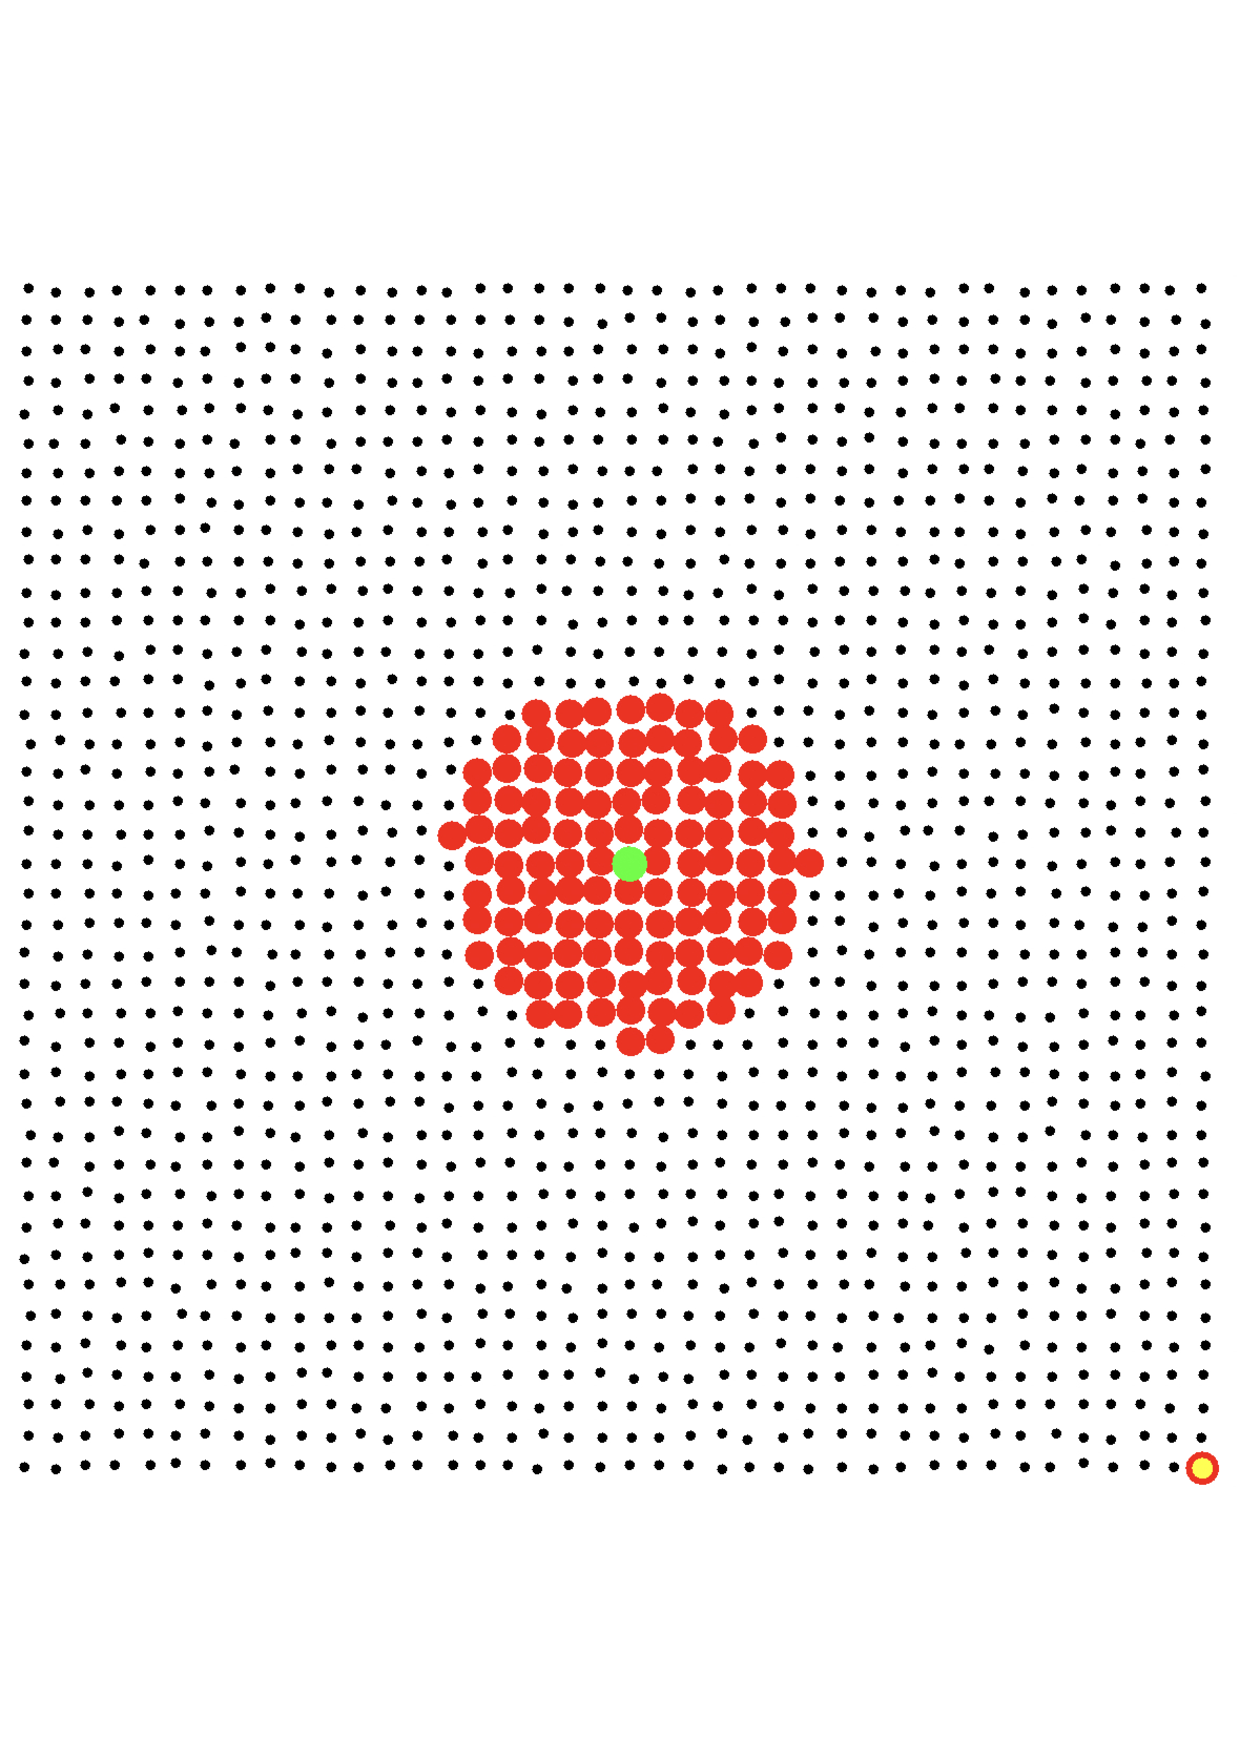
\includegraphics[width=.8\linewidth]{figures/in-circle-simulation.pdf}
    \caption{Simulazione dell'esperimento di InCircle in Alchemist.
    Il centro \texttt{o} è rappresentato dal dispositivo in verde, mentre i dispositivi
    all'interno del cerchio sono colorati in rosso.}
    \label{fig:in-circle-simulation}
\end{figure}

\section{Anello}
\label{sec:ring}



\section{Temperature}
\label{sec:temperature}

\section{Navigazione del Gradiente}
\label{sec:navgrad}

\section{Partizione di Voronoi}
\label{sec:voronoi}

\section{Connessione lungo l'albero di percorso minimo}
\label{sec:wire}

\section{Tracciamento}
\label{sec:track}

\section{Dinamica di uno stormo}
\label{sec:flock}







\backmatter


\bibliographystyle{alpha}
\bibliography{bibliography}

\begin{acknowledgements} % this is optional
Optional. Max 1 page.
\end{acknowledgements}

\end{document}
